\documentclass[a4paper, 12pt]{article}
\usepackage[dutch]{babel}
\usepackage{CJK}
\usepackage[CJK, overlap]{ruby} %furigana support
\usepackage{float}
\usepackage{graphicx}
\usepackage{multirow}
\usepackage{pdflscape}
\usepackage[left=2cm,top=1cm,right=2cm,bottom=2cm, nohead,nofoot]{geometry}

\renewcommand{\rubysize}{0.5}
\renewcommand{\rubysep}{-0.2ex}


\begin{document}

%%\begin{CJK*}[dnp]{JIS}{min}
\begin{CJK*}{UTF8}{min}
\CJKtilde
%\CJKcaption{JIS}

%
% Title page
%
\title{Aikibudo Terminologie}
\author{Andy Nagels}
\maketitle
\thispagestyle{empty} %should remove the page number
%\pagestyle{empty} %should remove the page number in the whole document
\begin{figure}[H]
\centering
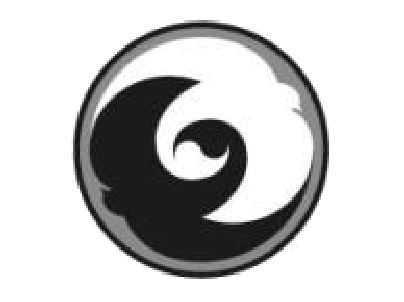
\includegraphics[width=2.5cm]{img/schild_aikibudo.eps}
\end{figure}

\begin{center}
合気武道
\end{center}

\begin{figure}[H]
\centering
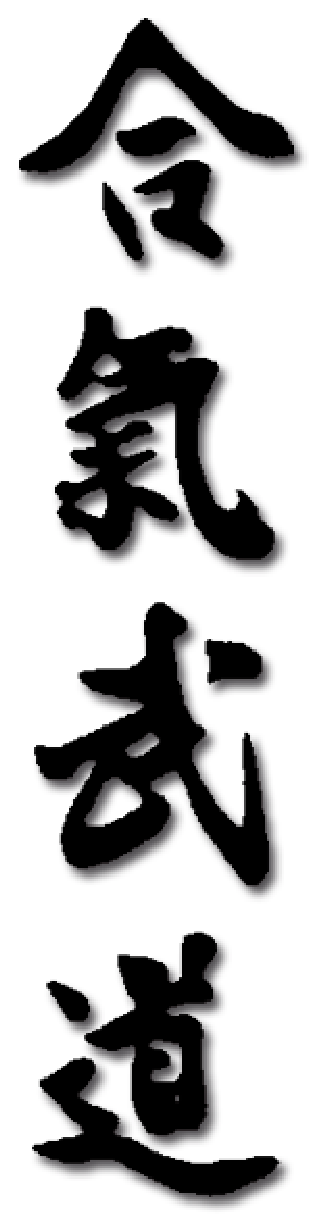
\includegraphics[width=1.0cm]{img/aikibudo-kanji.eps}
\end{figure}

%
% Disclaimer
%
\newpage
\begin{center}
\textbf{Disclaimer}\\
De vertalingen in dit document zijn gemaakt door mezelf, m.b.v. offici\"{e}le documenten, moderne technologie en mijn eigen kennis van het Japans. Daar ik echter geen expert ben in de Japanse taal, is het mogelijk dat er fouten staan in dit document. Naarmate mijn kennis van Aikibudo en Japans stijgt, zal ik de nieuwe kennis die ik heb opgedaan dan ook gebruiken om dit document na te kijken en te corrigeren.\\
Dit document is dus niet als finaal te beschouwen. Het wordt reeds vrijgegeven omdat het kan helpen bij het onthouden van de technieken.
\end{center}
\begin{center}
\textit{{\em Opmerking:} De laatste versie kan gratis gedownload worden van de
volgende url: http://c.dommel.be/aikibudo.html.}
\end{center}

%%%%%%%%%%%%%%%%%%%%%%%%%%%%%%%%%%%%%%
% Table of contents
%%%%%%%%%%%%%%%%%%%%%%%%%%%%%%%%%%%%%%
\newpage
\setcounter{page}{1}
\pagenumbering{Roman}
\tableofcontents

%%%%%%%%%%%%%%%%%%%%%%%%%%%%%%%%%%%%%%
% General info 
%%%%%%%%%%%%%%%%%%%%%%%%%%%%%%%%%%%%%%
\newpage
\setcounter{page}{1}
\pagenumbering{arabic}

% standard it's wadalab mincho, which gives the best results
%\CJKfamily{gothic}
\section{Inleiding}
\noindent Dit document bevat termen die gebruikt worden in aikibudo.

\section{De Japanse taal}
\noindent Alvorens we de berippen bekijken, dient een korte uitleg gegeven te worden over de Japanse taal.\\

\noindent Japans is opgebouwd uit 3 grote onderdelen: \textit{hiragana, katakana} en \textit{kanji}.\\

\noindent Hiragana en katakana zijn allebei een \textit{phonetisch} alfabet. Dat wil zeggen dat het symbolen voorstelt, die een klank uitbeelden.
Japans heeft dus geen aparte letters, zoals de meeste Westerse alfabetten.\\

\noindent \textbf{Hiragana} wordt gebruikt om zinnen te vormen en grammatica toe te passen op de Japanse taal. Het toont hoe Japans wordt uitgesproken.\\

\noindent \textbf{Katakana} bevat dezelfde klanken en enkele extra klanken. Het is ontstaan om de verschillende buitenlandse termen te kunnen uitspreken. Zo worden bvb. namen van niet Japanners in katakana geschreven.\\

\noindent \textbf{Kanji} zijn de meer complexe Japanse symbolen, die woorden en begrippen voorstellen. Ook Japanse namen en plaatsnamen worden meestal met kanji geschreven. Om te weten hoe deze symbolen worden uitgesproken, wordt gebruik gemaakt van hiragana, omdat hiragana een phonetisch alfabet is dat klanken in beeld brengt.\\

\noindent \textbf{Romaji} is een westerse schrijfwijze van Japanse klanken. Het wordt in Japan ook gebruikt om op een computer te typen.
Het is deze schrijfwijze, die het mogelijk maakt voor mensen die geen Japans kennen, om Japanse termen correct uit te spreken.

\noindent \textbf{Furigana} zijn kleine symbolen boven de kanji die in hiragana weergeven hoe de kanji moet worden uitgesproken.

\noindent In de tabel hieronder, kan je een overzicht vinden van de verschillende alfabetten, ter verduidelijking van bovenstaande uitleg.\\

\begin{table}[H]
\begin{center}
\begin{tabular}{c|c|c|c}
Nederlands alfabet & Hiragana & Katakana & Romaji\\
\hline
a &  あ & ア & a\\
k & bestaat niet & bestaat niet & bestaat niet\\
bestaat niet & か & カ & ka
\end{tabular}
\end{center}
\caption{Een kleine vergelijking ter verduidelijking}
\label{vergelijking_alfabetten}
\end{table}

\noindent De begrippen in dit document, zijn op volgende manier weergegeven:\\

\textit{Nederlandse omschrijving} $|$ \textit{Japanse term [met hiragana uitspraak boven de kanji]} $|$ \textit{romaji uitspraak}\\

\noindent De technieken zijn echter te lang om op die manier weer te geven. Zij staan dus onder elkaar:\\

\begin{center}
\textit{Nederlandse term}\\
\textit{Japanse term [met hiragana uitspraak boven de kanji]}\\
\textit{Romaji uitspraak}
\end{center}


%%%%%%%%%%%%%%%%%%%%%%%%%%%%%%%%%%%%%%
% Pronunciation
%%%%%%%%%%%%%%%%%%%%%%%%%%%%%%%%%%%%%%
\section{Uitspraak}
\noindent Een aantal letters worden iets anders uitgesproken in de romaji uitspraak, t.o.v. het Nederlands.
Het is interessant om dit even te lezen, om zo geen verkeerde uitspraak te leren voor de techniek.\\

\noindent j: $|zj|$ zoals in strand\textbf{j}anet, \textbf{J}efke, ... (en NIET zoals in \textbf{J}ommeke)\\
ch: $|tsj|$ zoals in \textbf{tsj}oeke \textbf{tsj}oeke tuut tuut\\
sh: $|sj|$ zoals in \textbf{ch}oco, \textbf{sh}ampoo, ...\\
u: korte $|oe|$ zoals in nen t\textbf{oe}k \textbf{oe}p aa bakkes, vake en m\textbf{oe}ke, ...\\
\={o} of ou: lange $|o|$ zoals in b\textbf{oo}t\\
\={u} of uu: lange $|u|$ zoals in v\textbf{uu}r

%%%%%%%%%%%%%%%%%%%%%%%%%%%%%%%%%%%%%%
% General terminology
%%%%%%%%%%%%%%%%%%%%%%%%%%%%%%%%%%%%%%
\section{Algemene terminologie}
\subsection{Algemeen}
\begin{table}[H]
\begin{center}
\begin{tabular}{c|c|c}
basis/oorsprong/standaard & \ruby{基本}{きほん} & kihon \\
\hline
de kunst van het veilig vallen & \ruby{受身}{うけみ} & ukemi \\
\hline
actieve partner & \ruby{取り}{どり} & dori\\
\hline
controle & \ruby{押}{お}さえ & osae\\
\hline
techniek & \ruby{技}{わざ} & waza\\
\hline
houding & \ruby{構}{かま}え & kamae 
\end{tabular}
\end{center}
\end{table}

\subsection{Richtingen en gebieden}
\begin{table}[H]
\begin{center}
\begin{tabular}{c|c|c}
rechts & \ruby{右}{みぎ} & migi \\
\hline
links & \ruby{左}{ひだり} & hidari\\
\hline
achterwaarts & \ruby{後}{うし}ろ & ushiro\\
\hline
voorwaarts & \ruby{前}{まえ} & mae\\
\hline
bovenste graad & \ruby{上段}{じょうだん} & j\={o}dan\\
\hline
midden & \ruby{中段}{ちゅうだん} & ch\={u}dan\\
\hline
grond & \ruby{土}{ど} & do
\end{tabular}
\end{center}
\end{table}

\subsection{Acties}
\begin{table}[H]
\begin{center}
\begin{tabular}{c|c|c}
worp & \ruby{投}{な}げ & nage\\
\hline
kopstoot & \ruby{頭突}{ずつ}き & zutsuki\\
\hline
trap & \ruby{蹴}{け}り & keri\\
\hline
wurging & \ruby{絞殺}{こうさつ} & k\={o}satsu\\
\hline
omkering/terug sturen & \ruby{返}{がえ}し & gaeshi\\
\hline
zijwaartse trap & \ruby{横蹴}{よこけ}り & yoko keri\\
\hline
stoot & \ruby{突}{つ}き & tsuki
\end{tabular}
\end{center}
\end{table}

\subsection{Lichaamsdelen}
\begin{table}[H]
\begin{center}
\begin{tabular}{c|c|c}
lichaam & \ruby{体}{たい} & tai \\
\hline
hand & \ruby{手}{て} & te \\
\hline
elleboog/elleboogstoot & \ruby{肘}{ひじ} & hiji\\
\hline
knie & \ruby{膝}{ひざ} & hiza\\
\hline
pols & \ruby{手首}{てくび} & tekubi\\
\hline
onderarm & \ruby{小手}{こて} & kote\\
\hline
schouder & \ruby{肩}{かた} & kata
\end{tabular}
\end{center}
\end{table}

\subsection{Andere begrippen}
\begin{table}[H]
\begin{center}
\begin{tabular}{c|c|c}
schroef/veer van horloge & \ruby{捻子}{ねじ} & neji\\
\hline
uitwendig & \ruby{表}{おもて} & omote\\
\hline
tabel & \ruby{表}{ひょう} & hy\={o}
\end{tabular}
\end{center}
\end{table}

\subsection{Leerstof}
\begin{table}[H]
\begin{center}
\begin{tabular}{c|c|c}
    verwijdering van het lichaam & \ruby{体捌}{たいさば}き & tai sabaki\\
\hline
valtechnieken & \ruby{受身技}{うけみわざ} & ukemi waza\\
\hline
stoottechnieken & \ruby{突}{つ}き\ruby{技}{わざ} & tsuki waza\\
\hline
traptechnieken & \ruby{蹴}{け}り\ruby{技}{わざ} & keri waza\\
\hline
? & ? [ほじょうんど] & hojo undo\\
\hline
vrij gevecht & \ruby{乱取}{らんど}り & randori
\end{tabular}
\end{center}
\end{table}

%%%%%%%%%%%%%%%%%%%%%%%%%%%%%%%%%%%%%%
% Kyuu techniques
%%%%%%%%%%%%%%%%%%%%%%%%%%%%%%%%%%%%%%
\newpage
\section{級の技 Ky\={u} technieken}
\subsection{6de ky\={u} [SHOKU]}
\begin{table}[H]
\begin{center}
\begin{tabular}{c|c}
\textbf{verwijdering van het lichaam} & ?\\
    \textbf{\ruby{体捌}{たいさば}き} & ? [いりみ]\\
\textbf{tai sabaki} & irimi\\
\cline{2-2}
& ?\\
& ? [おいりみ]\\
& o irimi\\
\hline
\textbf{valtechnieken} & achterwaarts\\
\textbf{\ruby{受身技}{うけみわざ}} & \ruby{後}{うし}ろ\\
\textbf{ukemi waza} & ushiro\\
\hline
\textbf{stoottechnieken} & ?\\
\textbf{\ruby{突}{つ}き\ruby{技}{わざ}} & ?\\
\textbf{tsuki waza} & ? \\
\hline
\end{tabular}
\end{center}
\label{kyuu_6}
\end{table}

\newpage
\subsection{5de ky\={u} [SHOKU]}
\subsubsection{Algemeen}
\subsubsection{技 Technieken}

\newpage
\subsection{4de ky\={u} [CHUKYU]}
\subsubsection{Algemeen}
\subsubsection{技 Technieken}

\newpage
\subsection{3de ky\={u} [CHUKYU]}
\subsubsection{Algemeen}
\subsubsection{技 Technieken}

\newpage
\subsection{2de ky\={u} [JOKYU]}
\subsubsection{Algemeen}
\subsubsection{技 Technieken}

\newpage
\subsection{1ste ky\={u} [JOKYU]}
\subsubsection{Algemeen}
\subsubsection{技 Technieken}

%%%%%%%%%%%%%%%%%%%%%%%%%%%%%%%%%%%%%%
% Dan techniques
%%%%%%%%%%%%%%%%%%%%%%%%%%%%%%%%%%%%%%
\newpage
\section{段の技 Dan technieken}
\subsection{第一段 1ste dan}
\subsubsection{Algemeen}
\begin{table}[H]
\begin{center}
\begin{tabular}{c}
zwarte gordel/persoon die een rang heeft\\
\ruby{有段者}{ゆうだんしゃ}\\
y\={u}dansha\\
\hline
1ste dan\\
\ruby{第一段}{だいいちだん}\\
daiichi dan
\end{tabular}
\end{center}
\label{dan_1_gen}
\end{table}

\subsubsection{技 Technieken}
\begin{table}[H]
\begin{center}
\begin{tabular}{c}
?\\
? [ひらき]\\
hiraki\\
\hline
weegschaal worp\\
\ruby{天秤投}{てんびんな}げ\\
tenbin nage\\
\hline
veer/schroef van horloge onderarm omkering\\
\ruby{螺子小手返}{ねじこてがえ}し\\
neji kote gaeshi\\
\hline
?\\
\ruby{螺子小手返}{ねじこてがえ}し\\
\end{tabular}
\end{center}
\label{dan_1}
\end{table}

\newpage
\subsection{2de dan}
\subsubsection{Algemeen}
\begin{table}[H]
\begin{center}
\begin{tabular}{c}
2de dan\\
\ruby{第二段}{だいにだん}\\
daini dan
\end{tabular}
\end{center}
\label{dan_2_gen}
\end{table}

\subsubsection{技 Technieken}

\newpage
\subsection{3de dan}
\subsubsection{Algemeen}
\begin{table}[H]
\begin{center}
\begin{tabular}{c}
3de dan\\
\ruby{第三段}{だいさんだん}\\
daisan dan
\end{tabular}
\end{center}
\label{dan_2_gen}
\end{table}

\subsubsection{技 Technieken}

%%%%%%%%%%%%%%%%%%%%%%%%%%%%%%%%%%%%%%
% Omote waza 
%%%%%%%%%%%%%%%%%%%%%%%%%%%%%%%%%%%%%%
\section{表技 Omote waza}

\newpage
\begin{landscape}
\thispagestyle{empty} %should remove the page number
\begin{center}
    \textbf{基本投げ技 Kihon nage waza (7 technieken)}
\end{center}
\addcontentsline{toc}{subsection}{\protect 基本投げ技 Kihon nage waza (7 technieken)}
\begin{table}[H]
\begin{center}
\scriptsize
\begin{tabular}{ccc}
\multicolumn{3}{c}{interval en ruimte laten - lijn van het lichaam}\\
\multicolumn{3}{c}{間合と間 - 体の線}\\
\multicolumn{3}{c}{ma ai to ma - tai no sen}\\
\\
(met) achterkant (vuist) (naar) zijkant van het gezicht slagen & naartoe gaan en neerslaan & achterwaartse val\\
\ruby{裏横面打}{うらよこめぬ}ち & \ruby{向}{むか}え\ruby{倒}{だお}し & \ruby{後受身}{うしろうけみ}\\
ura yoko men uchi & mukae daoshi & ushiro ukemi\\
\\
(met) voorkant (vuist) (naar) zijkant van het gezicht slagen & ? & achterwaartse val\\
\\
omote yoko men uchi & shiho nage & ushiro ukemi\\
\\
hoge stoot & elkaar kruisen & achterwaartse val\\
突き上段 & 行き違え & \ruby{後受身}{うしろうけみ}\\
tsuki j\={o}dan & yuki chigae & ushiro ukemi\\
\\
stoot naar het midden & veer/schroef van horloge onderarm omkering & voorwaartse val\\
\\
tsuki ch\={u}dan & neji kote gaeshi & mae ukemi\\
\\
? mouw vastpakken & ? & voorwaartse val\\
?\ruby{袖取}{りょうそでど}り  &   &   \\
ry\={o} sode dori & tenbin nage & mae ukemi\\
\\
? & ? & achterwaartse val\\
\\
do soku te dori & hachi mawashi & ushiro ukemi\\
\\
? handen vastpakken & heup worp & voorwaartse val\\
\\
ry\={o} te dori & koshi nage & mae ukemi
\end{tabular}
\end{center}
\label{kihonnagewaza}
\end{table}
\end{landscape}

\newpage
\thispagestyle{empty} %should remove the page number
\begin{landscape}
\begin{center}
    \textbf{基本押え技 Kihon osae waza (6 technieken)}
\end{center}
\addcontentsline{toc}{subsection}{\protect 基本押え技 Kihon osae waza (6 technieken)}
\begin{table}[H]
\begin{center}
\small
\begin{tabular}{ccc}
\multicolumn{3}{c}{interval en ruimte laten - lijn van het lichaam}\\
\multicolumn{3}{c}{間合と間 - 体の線}\\
\multicolumn{3}{c}{ma ai to ma - tai no sen}\\
\\
stoot op middenhoogte & in een achterwaartse beweging de elleboog breken & schouder gewricht\\
?[?] & ?[?] & ?[?]\\
tsuki ch\={u}dan & ushiro hiji kudaki & kata kansetsu
\\
(beide handen achter de rug vastpakken) & elleboog naar gezicht, opzij trekken na verlies evenwicht & schouder gewricht\\
ry\={o} te ippo dori & robuse & kata kansetsu\\
\\
(gi onder de schouder vastpakken) & pols breken & schouder gewricht\\
kata sode dori & kote kudaki & kata kansetsu\\
\\
\hline
\\
\multicolumn{3}{c}{interval en dichtbij - lijn van het lichaam}\\
\multicolumn{3}{c}{間合と近間 - 体の線}\\
\multicolumn{3}{c}{ma ai to chikama - tai no sen}\\
\\
\\
\\
ushiro kata dori & eri jime yuki chigae & ude kansetsu\\
\\
\\
ushiro ry\={o} te dori& shiho nage & kata kansetsu\\
\\
\\
ushiro uwate dori & mukae daoshi & kata kansetsu
\end{tabular}
\end{center}
\label{kihonosaewaza}
\end{table}
\end{landscape}

\newpage
\begin{center}
    \textbf{雄用技投げ技 Oy\={o} waza nage waza (間 - 近間)}
\end{center}
\addcontentsline{toc}{subsection}{雄用技投げ技 Oy\={o} waza nage waza (間 - 近間)}
\begin{table}[H]
\begin{center}
\begin{tabular}{c}
technieken voor mannen werp technieken(ruimte laten - dichtbij)\\
雄用技投げ技(間 - 近間)\\
oy\={o} waza nage waza (ma - chikama)\\
\end{tabular}
\end{center}
\label{oyouwazanagewaza}
\end{table}

\begin{center}
    \textbf{雄用技押え技 Oy\={o} waza osae waza (間 - 近間)}
\end{center}
\addcontentsline{toc}{subsection}{雄用技押え技 Oy\={o} waza osae waza (間 - 近間)}
\begin{table}[H]
\begin{center}
\begin{tabular}{c}
technieken voor mannen werp technieken(ruimte laten - dichtbij)\\
\ruby{雄用}{およう}\ruby{技}{わざ}\ruby{押}{おさ}え\ruby{技}{わざ}(\ruby{間}{ま} - \ruby{近間}{ちかま})\\
oy\={o} waza osae waza (ma - chikama)\\
\end{tabular}
\end{center}
\label{oyouwazaosaewaza}
\end{table}

\begin{center}
    \textbf{和の精神 Wa no sei shin}
\end{center}
\addcontentsline{toc}{subsection}{和の精神 Wa no sei shin}
\begin{table}[H]
\begin{center}
\begin{tabular}{c}
geest in harmonie\\
\ruby{和}{わ}の\ruby{精神}{せいしん}\\
wa no sei shin\\
\hline
voorwaarts en achterwaarts - lijn van het lichaam\\
前 と 後 - 体の線\\
mae to ushiro - tai no sen
\end{tabular}
\end{center}
\label{wanoseishin}
\end{table}

\begin{center}
    \textbf{乱取り Randori}
\end{center}
\addcontentsline{toc}{subsection}{乱取り Randori}
\begin{table}[H]
\begin{center}
\begin{tabular}{c}
vrij gevecht\\
乱取り[らんどり]\\
randori\\
\hline
zacht gevecht (ruimte laten - lijn van het lichaam)\\
\ruby{柔}{じゅう}の\ruby{乱取}{らんど}り (\ruby{間}{ま} - \ruby{体}{たい}の\ruby{線}{せん}) \\
j\={u} no randori (ma - tai no sen)
\end{tabular}
\end{center}
\label{randori}
\end{table}

\begin{center}
    \textbf{形大東流 - ? Kata dait\={o} ry\={u} - ikajo}
\end{center}
\addcontentsline{toc}{subsection}{形大東流 - ? Kata dait\={o} ry\={u} - ikajo}

%%%%%%%%%%%%%%%%%%%%%%%%%%%%%%%%%%%%%%
% Katori
%%%%%%%%%%%%%%%%%%%%%%%%%%%%%%%%%%%%%%
\newpage
\section{Tenshin Sh\={o}den Katori Shint\={o} Ry\={u}}
\subsection{Algemeen}
\begin{table}[H]
\begin{center}
\begin{tabular}{c}
de weg van de hemel gewijdt aan de positieve legende van het Katori altaar\\ 
%TODO: see if the katori furigana are with the correct kanji!
\ruby{天真}{てんしん}\ruby{正傳}{しょうでん}\ruby{香}{かとり}\ruby{取神}{しんとう}\ruby{道流}{りゅう}\\
tenshin sh\={o}den katori shint\={o} ry\={u}
\end{tabular}
\end{center}
\label{katori}
\end{table}


\subsection{6de ky\={u}}
\subsubsection{構え kamae}
\begin{table}[H]
\begin{center}
\begin{tabular}{c}
bovenste/hoge houding\\
\ruby{上段}{じょうだん}の\ruby{構}{かま}え\\
j\={o}dan no kamae\\
\hline
houding met de katana gericht naar de ogen van de tegenstander\\
\ruby{青眼}{せいがん}の\ruby{構}{かま}え\\
seigan no kamae\\
\hline
boog onder een hoek\\
\ruby{弧}{こ}がすみ\\
ko gasumi\\
\hline
hand naar achteren onder een hoek\\
\ruby{手裏}{てうらあ}がすみ\\
te ura gasumi\\
\hline
rechter lagere houding\\
\ruby{右下段}{みぎげだん}の\ruby{構}{かま}え\\
migi gedan no kamae\\
\hline
linker lagere houding (omgekeerde lagere)\\
\ruby{左下段}{ひだりげだん}の\ruby{構}{おかま}え\\
hidari gedan no kamae (gyaku gedan)\\
\hline
schaduw houding\\
\ruby{陰}{いん}の\ruby{構}{かま}え\\
in no kamae\\
\hline
schuine houding\\
\ruby{斜}{しゃ}の\ruby{構}{かま}え\\
sha no kamae\\
\hline
rechter hoge houding\\
\ruby{右上段}{みぎじょうだん}の\ruby{構}{かま}え\\
migi j\={o}dan no kamae\\
\hline
linker hoge houding\\
\ruby{左上段}{ひだりじょうだん}の\ruby{構}{かま}え\\
hidari j\={o}dan no kamae\\
\hline
? houding\\
? [しんのかまえ]\\
shin no kamae\\
\hline
? onder een hoek\\
? [おがすみ]\\
o gasumi\\
\hline
lager zitten (in houding)\\
\ruby{座}{すわ}り\ruby{下段}{げだん}(の\ruby{構}{かま}え)\\
suwari gedan (no kamae)\\
\hline
vogelstand\\
\ruby{鳥}{とり}\\
tori
\end{tabular}
\end{center}
\label{kyuu_6_katori_kamae}
\end{table}

\subsubsection{技 Technieken}
\noindent Alleen en in kumitachi.
\begin{table}[H]
\begin{center}
\begin{tabular}{c}
uitrol van een winding\\
\ruby{巻き打}{まきう}ち\\
maki uchi\\
\hline
uitrol zijkant van het gezicht\\
\ruby{横面打}{よこめんう}ち\\
yokomen uchi\\
\hline
uitrol naar de grond (volledige snijbeweging van boven naar onder)\\
\ruby{土打}{どう}ち\\
do uchi\\
\hline
bodem ontvangen\\
\ruby{土受}{どう}け\\
do uke\\
\hline
punt katana laten zakken en katana wegsteken\\
?[?]\\
noto
\end{tabular}
\end{center}
\label{kyuu_6_katori_other}
\end{table}

\subsection{5de ky\={u}}
\subsubsection{kata}
\begin{table}[H]
\begin{center}
\begin{tabular}{c}
?\\
?\\
ken no kata\\
\hline
?\\
?\\
bo no kata\\
\hline
?\\
?\\
kusanagi no ken (iai goshi)
\end{tabular}
\end{center}
\label{kyuu_5_katori_kata}
\end{table}

\subsubsection{bo jutsu}
\noindent Alleen en in kumitachi.
\begin{table}[H]
\begin{center}
\begin{tabular}{c}
?\\
?\\
yokomen uchi\\
\hline
?\\
?\\
do uchi\\
\hline
?\\
?\\
sune uchi
\end{tabular}
\end{center}
\label{kyuu_5_katori_bo}
\end{table}

\subsection{4de ky\={u}}
\subsubsection{kata}
\begin{table}[H]
\begin{center}
\begin{tabular}{c}
?\\
?\\
itsutsu no tachi (kiri komi)\\
\hline
?\\
?\\
nuki tsuke no ken (iai goshi)
\end{tabular}
\end{center}
\label{kyuu_4_katori_kata}
\end{table}

\subsection{3de ky\={u}}
\subsubsection{kata}
\begin{table}[H]
\begin{center}
\begin{tabular}{c}
?\\
?\\
nanatsu no tachi (kiri komi)\\
\hline
?\\
?\\
nuki uchi no ken (iai goshi)\\
\hline
?\\
?\\
seri ai no bo (uchi komi)
\end{tabular}
\end{center}
\label{kyuu_3_katori_kata}
\end{table}

\subsection{2de ky\={u}}
\subsubsection{kata}
\begin{table}[H]
\begin{center}
\begin{tabular}{c}
?\\
?\\
kasumi no tachi (kiri komi)\\
\hline
?\\
?\\
sune hishigi no bo (uchi komi)\\
\hline
?\\
?\\
itsutsu no naginata (kiri komi)\\
\hline
?\\
?\\
uken (iai goshi)
\end{tabular}
\end{center}
\label{kyuu_2_katori_kata}
\end{table}

\subsection{1ste ky\={u}}
\subsubsection{kata}
\begin{table}[H]
\begin{center}
\begin{tabular}{c}
?\\
?\\
haka no tachi (kiri komi)\\
\hline
?\\
?\\
saken (iai goshi)\\
\hline
?\\
?\\
happo ken (iai goshi)
\end{tabular}
\end{center}
\label{kyuu_1_katori_kata}
\end{table}

\subsection{第一段 1ste dan}
\subsubsection{kata}
\noindent Een perfecte kennis is vereist van alle voorgaande technieken.\\

\subsubsection{extra}
\begin{itemize}
\item Houding van het lichaam en perfectie van de posities: shisei
\item Uitgesproken expressie van kime, zanshin en kiai
\item Kennis van de kobudo termen en de verschillende onderdelen waaruit een katana is opgebouwd
\end{itemize}

\end{CJK*}
\end{document}
